\section{Stylized Facts}\label{sec:sf}

We document eight stylized facts on the 600-market panel
(Section~\ref{ssec:panel}). Each subsection reports a per-market
distribution and, where the data support one, a regression coefficient.
Underlying parquet artifacts are in the replication package.

\subsection{SF1 -- Longshot spread premium}\label{ssec:sf1}

We bin quoted half-spread (in basis points of mid) by per-market mean
mid price into ten deciles. Median spread is $\sim 400$\,bps in the
central $[0.4, 0.6]$ range and climbs to 1{,}300--1{,}800\,bps for
markets trading below $0.10$. The pattern is asymmetric: the
low-probability side is wider than the high-probability side, which
echoes the longshot bias documented in the racetrack and parimutuel
literature \citep{snowberg-wolfers-2010,thaler-ziemba-1988} and the
prediction-market longshot evidence on Iowa Electronic Markets and
TradeSports surveyed by \citet{wolfers-zitzewitz-2004}. The direction
is the same; the magnitude is not. Racetrack longshot premia are
typically a few percent of stake, and prediction-market longshot
biases observed on IEM and TradeSports run in the same range. The
1{,}300--1{,}800\,bps full quoted spread on Polymarket's lowest-
probability decile (i.e., 650--900\,bps half-spread) is an order
of magnitude wider, which reads less like the classical risk-love
or misperception story and more like a liquidity-provision
constraint: low-probability binary contracts
have a bounded upside and an asymmetric downside for the maker, so
the inventory-risk premium on the wide side is mechanically larger
than on a continuous-payoff sportsbook market. Distinguishing
inventory risk from a behavioural longshot premium would require
data we do not collect (maker realised inventory and time-on-book),
so we report SF1 as a Polymarket-specific quoted-spread stylised
fact and leave the structural decomposition to follow-on work.

\begin{figure}[htbp]
  \centering
  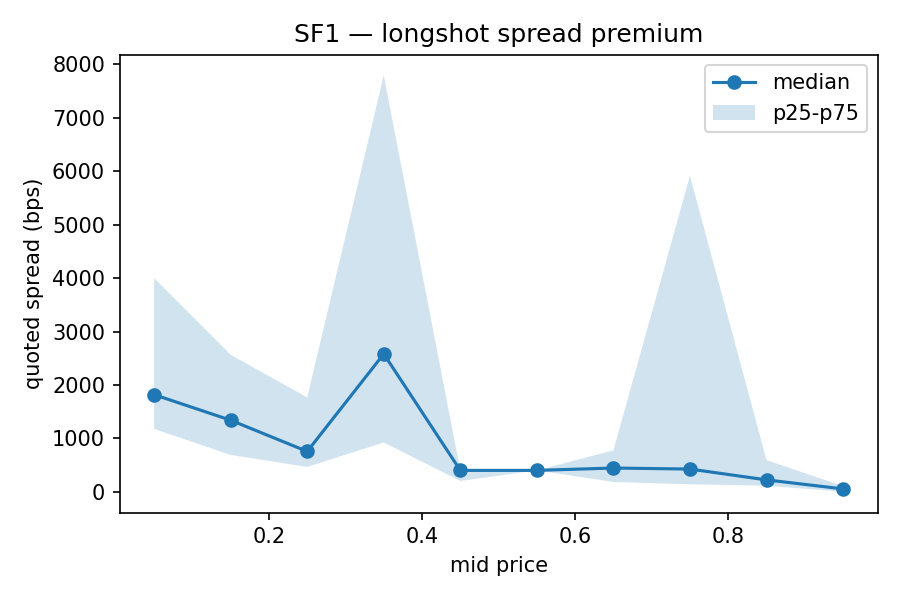
\includegraphics[width=0.95\columnwidth]{figures/sf1_longshot.png}
  \caption{SF1 panel: median quoted spread (bps) per mid-price decile,
    600 panel markets. Shaded band is interquartile range.}
  \label{fig:sf1}
\end{figure}

\begin{table*}[htbp]
  \centering
  \caption{SF1 panel — quoted spread by mid-price decile.}
  \label{tab:sf1_longshot}
  \begin{tabular}{lrrrrrr}
\toprule
Bin & Mid lo & Mid hi & Markets & Median (bps) & p25 (bps) & p75 (bps) \\
\midrule
0 & 0.0000 & 0.1000 & 33 & 1,818 & 1,176 & 4,000 \\
1 & 0.1000 & 0.2000 & 18 & 1,339 & 689.66 & 2,564 \\
2 & 0.2000 & 0.3000 & 18 & 754.99 & 465.12 & 1,767 \\
3 & 0.3000 & 0.4000 & 21 & 2,581 & 923.08 & 7,797 \\
4 & 0.4000 & 0.5000 & 184 & 400.00 & 202.02 & 400.00 \\
5 & 0.5000 & 0.6000 & 214 & 400.00 & 400.00 & 400.00 \\
6 & 0.6000 & 0.7000 & 27 & 444.44 & 183.49 & 775.19 \\
7 & 0.7000 & 0.8000 & 12 & 425.09 & 139.86 & 5,915 \\
8 & 0.8000 & 0.9000 & 15 & 222.22 & 114.29 & 591.72 \\
9 & 0.9000 & 1.00 & 4 & 53.48 & 0.0000 & 106.95 \\
\bottomrule
\end{tabular}

\end{table*}

\subsection{SF2 -- Depth concentration}\label{ssec:sf2}

We summarize the L2 depth profile by the ratio
$\mathrm{depth}_{L=1} / \mathrm{depth}_{L=10}$, the share of cumulative
top-10 depth held at the top-of-book. A value of $1.0$ means the
entire top-10 depth sits at level 1 (a thin, top-heavy book); $0.1$
matches a uniform grid where each level carries equal depth.

For the 546 markets with non-null depth, the median ratio is
\textbf{0.137}, close to the uniform-grid benchmark, with
$p_{10}=0.033$ and $p_{90}=0.428$. The folk view that
prediction-market books are concentrated at top-of-book does not hold
on Polymarket: depth is generally layered deeper into the book, with a
right tail of markets where the top-of-book share approaches one.

\begin{figure}[htbp]
  \centering
  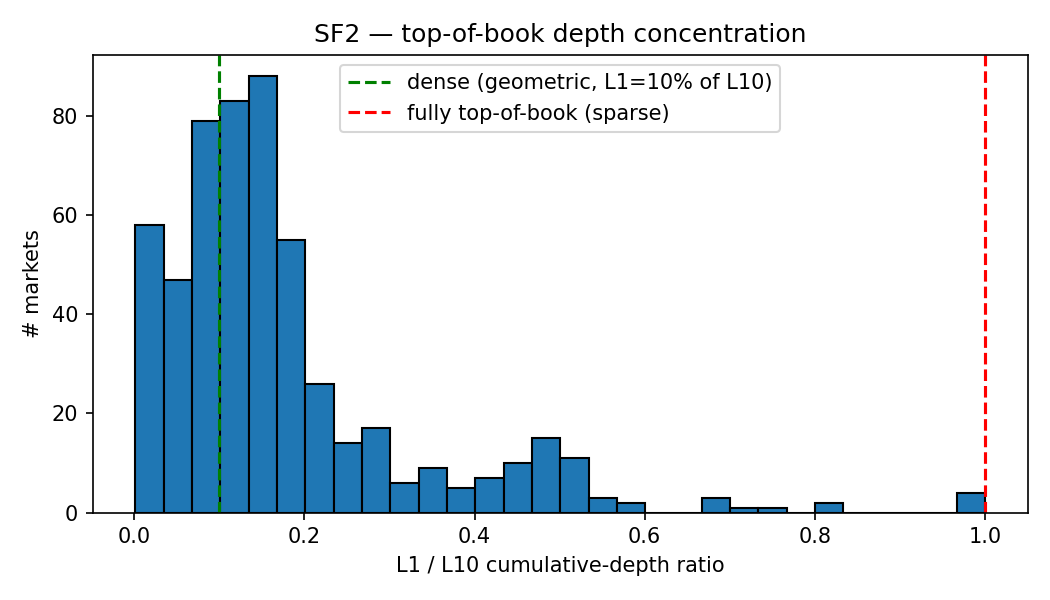
\includegraphics[width=0.95\columnwidth]{figures/sf2_depth_profile.png}
  \caption{SF2 panel: histogram of $L_1/L_{10}$ depth-concentration ratio
    across 546 panel markets. Vertical lines mark the uniform-grid
    benchmark (green, $0.10$) and the fully top-of-book limit (red, $1.0$).}
  \label{fig:sf2}
\end{figure}

\subsection{SF3 -- Polygon block-clock alignment}\label{ssec:sf3}

We test whether \texttt{price\_change} events cluster near Polygon block
boundaries by computing, per market, the share of events that fall
within $\pm 100$\,ms of the nearest 2\,000\,ms grid point. Under a
uniform-timing null this share is $0.10$.

The panel-level distribution sits tight against the null: median
\textbf{0.102} with interquartile range $[0.087, 0.110]$; only
27 markets (4.5\%) lie above a 0.15 threshold. At the per-market
level, however, a two-sided binomial test of $H_0$:~share~$=0.10$
rejects in \textbf{351 of 600 markets} (58.5\%) at $\alpha=0.05$.
That high rejection rate is a mechanical consequence of large
event counts: millions of events per market make the binomial test
sensitive to tiny deviations from 0.10. The economic interpretation
is that quote-timing does \emph{not} cluster on block boundaries to
a meaningful degree, even though high-volume markets reject the
exact point null statistically.

\begin{figure}[htbp]
  \centering
  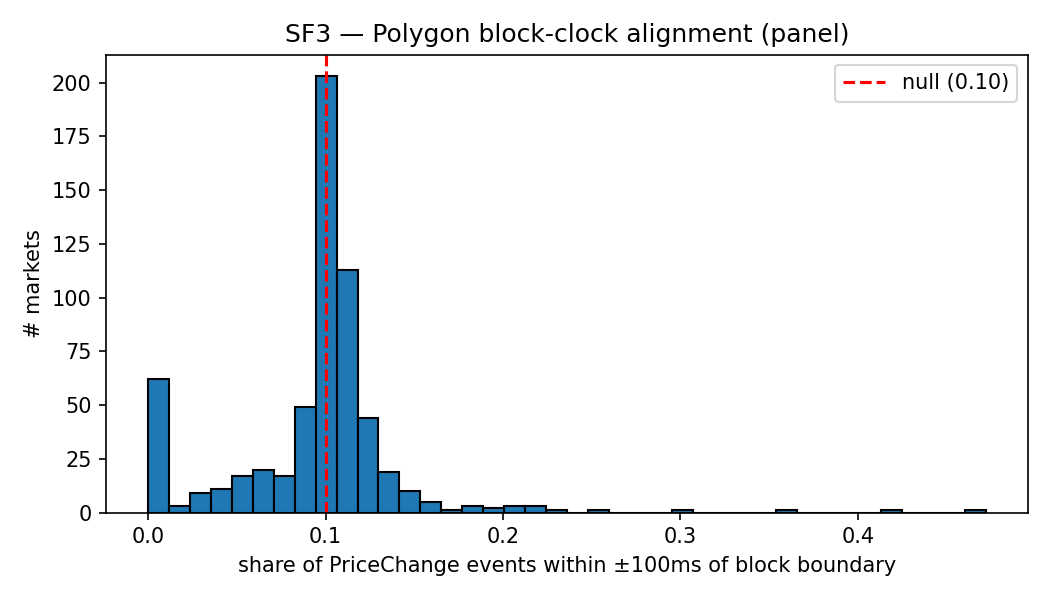
\includegraphics[width=0.95\columnwidth]{figures/sf3_blockclock.png}
  \caption{SF3 panel: distribution of per-market block-alignment shares.
    The red dashed line marks the chance-level null ($0.10$).}
  \label{fig:sf3}
\end{figure}

\subsection{SF4 -- Maker-wallet concentration}\label{ssec:sf4}

For each market we compute the volume-weighted Herfindahl index (HHI)
of maker-address share across on-chain trades in the scrape window. A
single dominant maker yields $\mathrm{HHI}=1$; a uniform distribution
across $n$ makers yields $1/n$.

Across 600 markets and 6.4\,M trades, the median HHI is \textbf{0.031}
($\sim 32$ effective makers). The distribution is right-skewed:
$p_{90}=0.119$ ($\sim 8$ effective makers) and a maximum of $0.40$
(roughly 3 effective makers). Maker liquidity is decentralised on most
markets in the panel, with a tail of thin or niche markets dominated
by one to three wallets.

\begin{figure}[htbp]
  \centering
  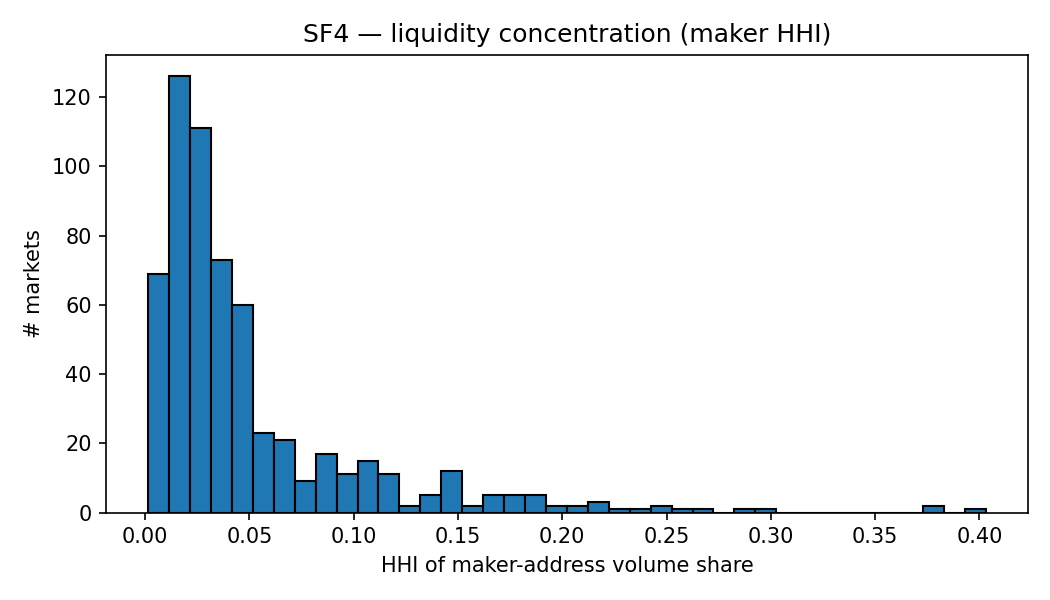
\includegraphics[width=0.95\columnwidth]{figures/sf4_herfindahl.png}
  \caption{SF4 panel: distribution of per-market maker-address Herfindahl
    indices across 600 markets.}
  \label{fig:sf4}
\end{figure}

\subsection{SF5 -- Category-conditional spread}\label{ssec:sf5}

Per-market metadata is pulled from CLOB REST and questions are
keyword-classified into a small bucket scheme. Politics, Business, and
Entertainment buckets each had fewer than ten panel markets and were
merged into Other for statistical reliability, leaving four
categories: Crypto (348/600, 58\%), Sports (142/600, 24\%), Other
(75/600), Geopolitics (35/600). For the on-chain effective half-spread
the medians (in probability points) are reported in
Table~\ref{tab:sf5_category} and visualised in
Figure~\ref{fig:sf5}.

\begin{table*}[htbp]
  \centering
  \caption{SF5 panel — effective half-spread by keyword-derived category.}
  \label{tab:sf5_category}
  \begin{tabular}{lrrrr}
\toprule
Category & Markets & Median half-spread (prob pp) & p25 & p75 \\
\midrule
Sports & 142 & 0.0075 & -0.1087 & 0.2201 \\
Geopolitics & 35 & 0.0001 & -0.0014 & 0.0206 \\
Other & 75 & -0.0004 & -0.0596 & 0.0456 \\
Crypto & 348 & -0.0393 & -0.2494 & 0.0968 \\
\bottomrule
\end{tabular}

\end{table*}

\begin{figure}[htbp]
  \centering
  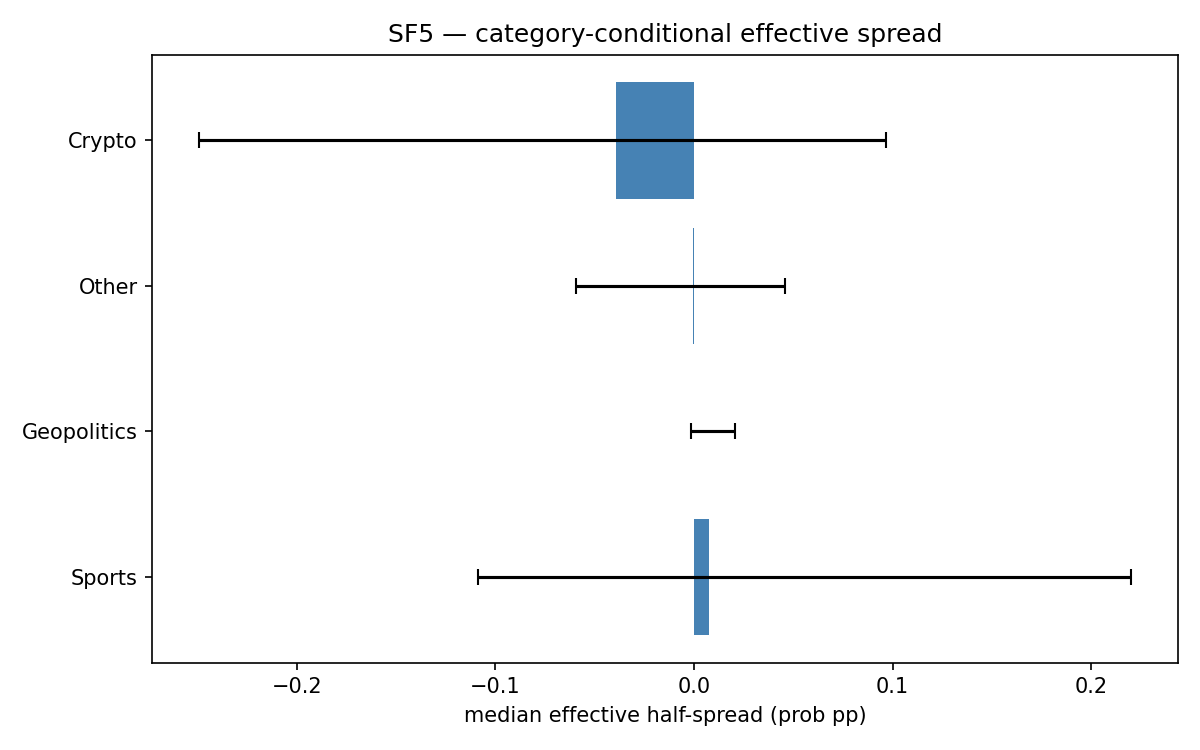
\includegraphics[width=0.95\columnwidth]{figures/sf5_category.png}
  \caption{SF5 panel: median effective half-spread by category, with
    interquartile-range error bars. Categories are derived from
    keyword classification of CLOB REST \texttt{question} text.}
  \label{fig:sf5}
\end{figure}

Cross-category dispersion of medians is small in absolute terms (all
within $\pm 0.04$ probability points), but within-category
interquartile ranges are wide for Crypto and Sports
($p_{75} - p_{25}\approx 0.3$\,prob.~pp). The wide within-category
spread is consistent with the measurement noise documented in
Section~\ref{sec:limits}.

\subsection{SF6 -- Archive-ingestion latency}\label{ssec:sf6}

Each archive row carries two timestamps:
\texttt{timestamp\_received} (exchange side) and
\texttt{timestamp\_created\_at} (collector side). Their difference is
a per-event ingestion delay. Across 547 markets with non-empty
windows, the median per-market $p_{50}$ delay is \textbf{41.5\,ms},
with $p_{90}=166$\,ms and $p_{99}=6{,}108$\,ms. The inter-market
spread of $p_{50}$ is tight ($p_{25}$--$p_{75}$: 39--47\,ms), which
points to collector-pipeline behaviour rather than trader latency.
The $p_{99}$ tail of several seconds points to occasional
backpressure events at the collector.

\begin{figure}[htbp]
  \centering
  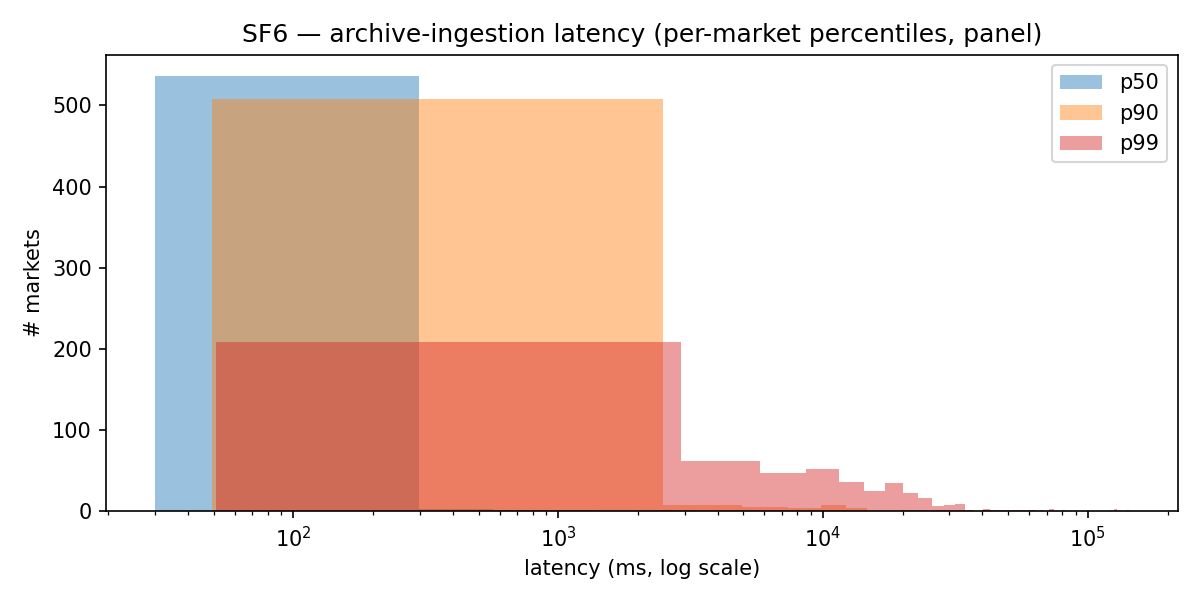
\includegraphics[width=0.95\columnwidth]{figures/sf6_latency.png}
  \caption{SF6 panel: per-market percentile distributions of
    archive-ingestion latency (log scale).}
  \label{fig:sf6}
\end{figure}

\subsection{SF7 -- Self-counterparty wash share}\label{ssec:sf7}

We flag a trade as wash-suspect under a two-tier rule:
(a) \texttt{maker == taker} (direct self-match), or
(b) a flipped pair $(\mathrm{maker}_a, \mathrm{taker}_a) \leftrightarrow
(\mathrm{taker}_a, \mathrm{maker}_a)$ within 128 blocks
(Polygon finality buffer) on the same market. This is an explicit
\emph{lower bound}: it captures only direct and immediate-roundtrip
self-counterparty patterns, not the extended-graph patterns that
network-based classifiers such as \citet{cong-li-niu-2023} address
on unregulated cryptocurrency token exchanges, where wash shares of
25--70\% have been documented. We cite this range as a sanity bound,
not an apples-to-apples reference: the wash-incentive environment on
token exchanges (listing-fee thresholds, aggregator-ranking
optimisation, volume-tied market-making rebates) differs from the
incentive environment on a prediction market that resolves into a
single binary payoff and does not list across competing aggregators.

Across 600 markets and 6.4\,M trades, the median wash share is
\textbf{0.97\%}, with $p_{90}=4.5\%$, $p_{99}=10.6\%$, and a maximum
of 22.2\%. The gap between our lower bound and the network-classifier
estimates on token exchanges has two components: wash patterns that
require multi-counterparty graph analysis to detect (which our
detector does not cover), plus a venue-class difference in the
underlying wash incentives. We can quantify the first component only
under a graph-classifier extension; the second component is
identification, not measurement.

\begin{figure}[htbp]
  \centering
  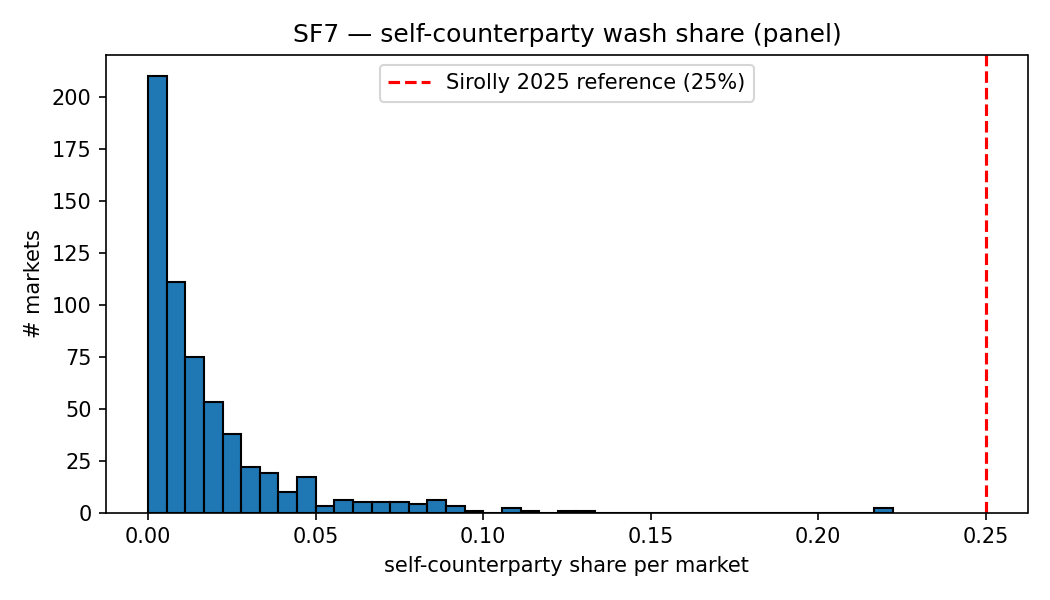
\includegraphics[width=0.95\columnwidth]{figures/sf7_wash.png}
  \caption{SF7 panel: distribution of self-counterparty wash share by
    market. Red dashed line marks a 25\% reference, the lower bound
    of the wash-share range documented by \citet{cong-li-niu-2023}
    on unregulated cryptocurrency venues.}
  \label{fig:sf7}
\end{figure}

\subsection{SF8 -- Depth decay near resolution}\label{ssec:sf8}

Do markets near resolution carry shallower books? We regress log mean
depth at $L=10$ on log seconds-to-close at the panel window midpoint
(2026-03-13), restricted to 322 markets with positive seconds-to-close
and non-zero summary depth.

\begin{table}[htbp]
  \centering
  \caption{SF8 — cross-sectional panel regression of log mean depth on
    log seconds-to-close. HC3-robust standard error.}
  \label{tab:sf8_depth_decay}
  \scriptsize
  \begin{tabular}{lrrr}
\toprule
Markets in fit & Slope on log(ttc) & SE (HC3) & R² \\
\midrule
322 & 0.8178 & 0.1133 & 0.1293 \\
322 & 0.5500 & 0.1429 & 0.2165 \\
322 & 0.3048 & 0.1036 & 0.4857 \\
\bottomrule
\end{tabular}

\end{table}

The bivariate slope is \textbf{0.818} (HC3 SE 0.113, $t=7.2$,
$R^2 = 0.13$). Category fixed effects (Crypto, Sports, Other,
Geopolitics) attenuate the slope to \textbf{0.550} (HC3 SE 0.143,
$t=3.85$, $R^2=0.22$): roughly a third of the bivariate association
is category-level confounding. Adding log panel-window volume on top
of category attenuates further to \textbf{0.305} (HC3 SE 0.104,
$t=2.94$, $R^2=0.49$). Volume absorbs much of the cross-sectional
depth variation, but the time-to-close coefficient stays positive
and significant. A 0.31 slope works out to $\sim 6\%$ less mean
depth per $10\times$ reduction in seconds-to-close, a smaller
economic magnitude than the bivariate or the category-FE
specification implied. The category + log-volume
specification is the conservative reading. Volume mediates the
depth-time relationship because markets active longer accumulate
more makers, and more makers means more depth, so a regression that
omits volume attributes the makers-and-time channel to time alone.
The 0.305 coefficient is the residual depth decay after that
mediation is netted out; the 0.550 within-category slope reported in
the abstract and intro is the figure before mediation is netted out
and is the appropriate one to compare to a literature that does not
condition on volume.

\begin{figure}[htbp]
  \centering
  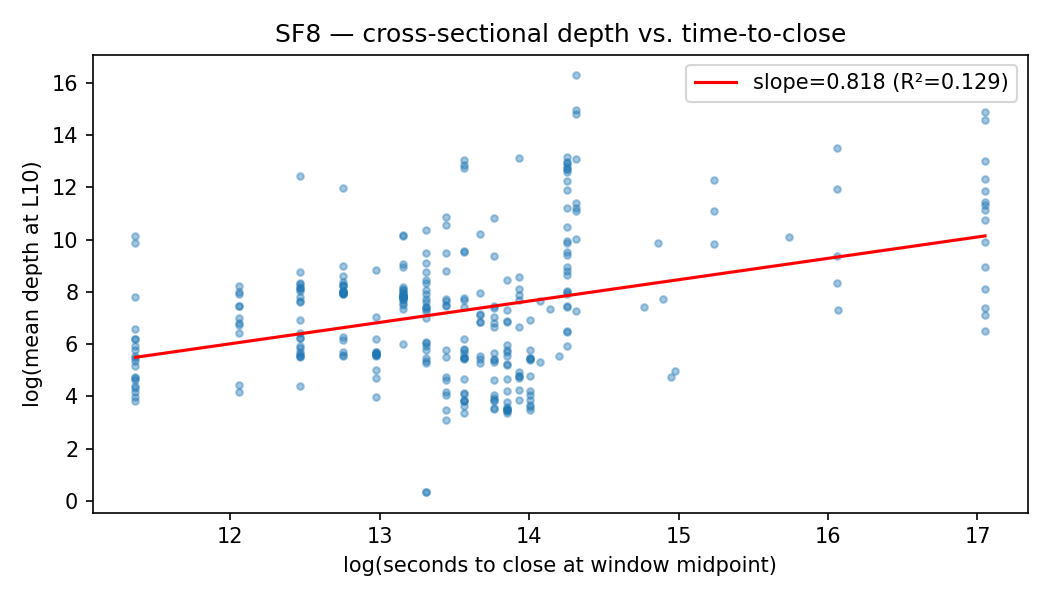
\includegraphics[width=0.95\columnwidth]{figures/sf8_depth_decay.png}
  \caption{SF8: cross-sectional fit of log mean depth on log
    seconds-to-close at the panel midpoint.}
  \label{fig:sf8}
\end{figure}
